\begin{pastexam}[label={px:df3-112-ds-03}]{地方三等資訊處理 112 年 第三題}
（申論；10 分）

請以如下的 Huffman Tree 所做的數字編碼，解讀 01010111110100100011 編碼對應的數字。（10 分）
\begin{center}
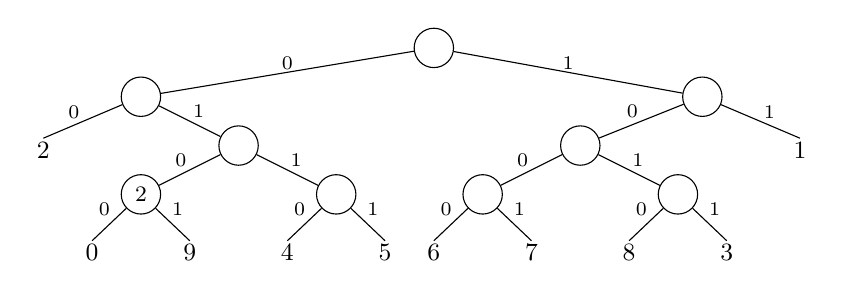
\begin{tikzpicture}[x=0.62cm, y=0.62cm,
  n/.style={circle, draw, minimum size=5mm, inner sep=0pt, font=\footnotesize},
  l/.style={font=\small},
  b/.style={font=\scriptsize, inner sep=1pt}]
\node[n] (R) at (8,0) {};
\node[n] (L) at (2,-1) {};
\node[n] (Rt) at (13.5,-1) {};
\node[l] (two) at (0,-2.1) {2};
\node[n] (L1) at (4,-2) {};
\node[n] (R0) at (11,-2) {};
\node[l] (one) at (15.5,-2.1) {1};
\node[n] (A) at (2,-3) {2};
\node[n] (B) at (6,-3) {};
\node[n] (C) at (9,-3) {};
\node[n] (D) at (13,-3) {};
\foreach \p/\x/\t in {A/1/0, A/3/9, B/5/4, B/7/5, C/8/6, C/10/7, D/12/8, D/14/3} {
  \node[l] (\t x\x) at (\x,-4.2) {\t};
  \draw (\p) -- (\x,-3.95);
}
\draw (R) -- node[b, above] {0} (L);
\draw (R) -- node[b, above] {1} (Rt);
\draw (L) -- node[b, above left] {0} (0,-1.85);
\draw (L) -- node[b, above right] {1} (L1);
\draw (Rt) -- node[b, above left] {0} (R0);
\draw (Rt) -- node[b, above right] {1} (15.5,-1.85);
\draw (L1) -- node[b, above left] {0} (A);
\draw (L1) -- node[b, above right] {1} (B);
\draw (R0) -- node[b, above left] {0} (C);
\draw (R0) -- node[b, above right] {1} (D);
\foreach \x/\y/\lab in {1.25/-3.3/0, 2.75/-3.3/1, 5.25/-3.3/0, 6.75/-3.3/1, 8.25/-3.3/0, 9.75/-3.3/1, 12.25/-3.3/0, 13.75/-3.3/1}
  \node[b] at (\x,\y) {\lab};
\end{tikzpicture}
\end{center}
\end{pastexam}

\begin{pastsoln}
原圖左下有一個內部節點的圓圈裡寫著「2」，其他內部節點都是空白的。 它有兩個子節點（$0$ 和
$9$），是內部節點，那個「2」應該是誤植，不影響解碼。

\textbf{先讀出每個數字的編碼}：從根走到葉子，往左記 $0$、往右記 $1$。
\begin{center}
\begin{tabular}{cc|cc|cc|cc|cc}
\toprule
數字 & 編碼 & 數字 & 編碼 & 數字 & 編碼 & 數字 & 編碼 & 數字 & 編碼 \\
\midrule
2 & 00 & 0 & 0100 & 9 & 0101 & 4 & 0110 & 5 & 0111 \\
1 & 11 & 6 & 1000 & 7 & 1001 & 8 & 1010 & 3 & 1011 \\
\bottomrule
\end{tabular}
\end{center}
霍夫曼碼是前綴碼：沒有一個編碼是另一個編碼的開頭（每個數字都在葉子上），所以從頭讀，
一走到葉子就確定一個數字，再回到根繼續，不會有歧義（資結書第~19.3~節）。

\textbf{解碼} $01010111110100100011$（共 $20$ 位元）：
\begin{center}
\begin{tabular}{clll}
\toprule
段 & 讀到的位元 & 在樹上的路徑 & 數字 \\
\midrule
1 & 0101 & 左、右、左、右 & 9 \\
2 & 0111 & 左、右、右、右 & 5 \\
3 & 11 & 右、右 & 1 \\
4 & 0100 & 左、右、左、左 & 0 \\
5 & 1000 & 右、左、左、左 & 6 \\
6 & 11 & 右、右 & 1 \\
\bottomrule
\end{tabular}
\end{center}
$4 + 4 + 2 + 4 + 4 + 2 = 20$ 位元剛好用完，沒有剩下的位元。 對應的數字是
\[
\mathbf{9\ 5\ 1\ 0\ 6\ 1}.
\]
\end{pastsoln}
